\section{Anhang}

\subsection{Trigonometie}

% Copy-Paste from KomFour

\begingroup
\renewcommand{\arraystretch}{2}
\setlength{\tabcolsep}{0mm}
\scalebox{0.33}{
\Huge
\begin{tabularx}{3\columnwidth}{rp{1mm}V{3}*{17}{C}}
    \rowcolor{subsectioncolor!30}$\bm{\alpha}$\phantom{${}^{\circ}$} && $0$ & $\dfrac{\pi}{6\mathstrut}$ & $\dfrac{\pi}{4}$ & $\dfrac{\pi}{3}$ & $\dfrac{\pi}{2}$ & $\dfrac{2\pi}{3}$ & $\dfrac{3\pi}{4}$ & $\dfrac{5\pi}{6}$ & $\pi$ & $\dfrac{7\pi}{6}$ & $\dfrac{5\pi}{4}$ & $\dfrac{4\pi}{3}$ & $\dfrac{3\pi}{2}$ & $\dfrac{5\pi}{3}$ & $\dfrac{7\pi}{4}$ & $\dfrac{11\pi}{6}$ & $2\pi$ \\\hline
    \rowcolor{subsectioncolor!30}$\bm{\alpha^\circ}$ && \phantom{${}^\circ$}$0^\circ$ & $30^\circ$ & $45^\circ$ & $60^\circ$ & $90^\circ$ & $120^\circ$ & $135^\circ$ & $150^\circ$ & $180^\circ$ & $210^\circ$ & $225^\circ$ & $240^\circ$ & $270^\circ$ & $300^\circ$ & $315^\circ$ & $330^\circ$ & $360^\circ$ \\\hline
    $\bm{\sin(\alpha)}$ && $0$ & $\dfrac{1}{2\mathstrut}$ & $\dfrac{\sqrt{2}}{2}$ & $\dfrac{\sqrt{3}}{2}$ & $1$ & $\dfrac{\sqrt{3}}{2}$ & $\dfrac{\sqrt{2}}{2}$ & $\dfrac{1}{2}$ & $0$ & $-\dfrac{1}{2}$ & $-\dfrac{\sqrt{2}}{2}$ & $-\dfrac{\sqrt{3}}{2}$ & $-1$ & $-\dfrac{\sqrt{3}}{2}$ & $-\dfrac{\sqrt{2}}{2}$ & $-\dfrac{1}{2}$ & $0$ \\\hline
    $\bm{\cos(\alpha)}$ && $1$ & $\dfrac{\sqrt{3}}{2\mathstrut}$ & $\dfrac{\sqrt{2}}{2}$ & $\dfrac{1}{2}$ & $0$ & $-\dfrac{1}{2}$ & $-\dfrac{\sqrt{2}}{2}$ & $-\dfrac{\sqrt{3}}{2}$ & $-1$ & $-\dfrac{\sqrt{3}}{2}$ & $-\dfrac{\sqrt{2}}{2}$ & $-\dfrac{1}{2}$ & $0$ & $\dfrac{1}{2}$ & $\dfrac{\sqrt{2}}{2}$ & $\dfrac{\sqrt{3}}{2}$ & $1$ \\\hline
    $\bm{\tan(\alpha)}$ && $0$ & $\dfrac{\sqrt{3}}{3\mathstrut}$ & $1$ & $\sqrt{3}$ & $\pm\infty$ & $-\sqrt{3}$ & $-1$ & $-\dfrac{\sqrt{3}}{3}$ & $0$ & $\dfrac{\sqrt{3}}{3}$ & $1$ & $\sqrt{3}$ & $\pm\infty$ & $-\sqrt{3}$ & $-1$ & $-\dfrac{\sqrt{3}}{3}$ & $0$ \\\hline
    $\bm{\cot(\alpha)}$ && $\pm\infty$ & $\sqrt{3}$ & $1$ & $\dfrac{\sqrt{3}}{3\mathstrut}$ & $0$ & $-\dfrac{\sqrt{3}}{3}$ & $-1$ & $-\sqrt{3}$ & $\pm\infty$ & $\sqrt{3}$ & $1$ & $\dfrac{\sqrt{3}}{3}$ & $0$ & $-\dfrac{\sqrt{3}}{3}$ & $-1$ & $-\sqrt{3}$ & $\pm\infty$ \\
\end{tabularx}}
\endgroup


\subsection{Bodediagramm eines Integrators}
\label{Bodediagramm eines Integrators}

Ein Integrator mit $G(s) = \frac{K}{s}$ hat seine Polstelle bei der Frequenz $\omega = 0$. Im Bodediagramm wird der Integrator so
dargestellt, dass bei Frequenz $\omega = 1$ die Verstärkung $20 \, \deci \bel \cdot \log_{10}(K)$ erreicht ist. 
Die Steigung beträgt $-20 \, \deci \bel / \mathrm{Dek}$ und die Phase ist konstant bei $\varphi = -\frac{\pi}{2}$

\begin{center}
    % Gain
    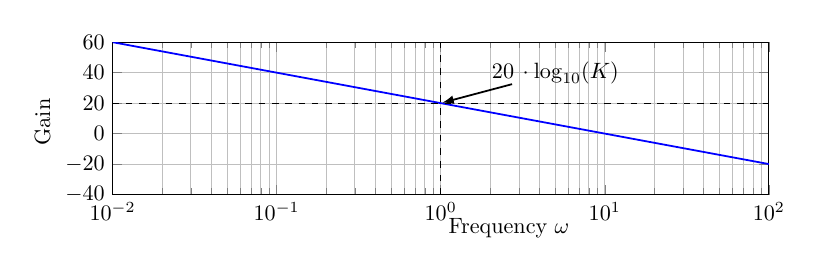
\begin{tikzpicture}
        [
            scale = 0.8,
            >=latex
        ]
        \begin{axis}
            [
                width=12cm,
                height=4cm,
                xmode=log,
                xmin=0.01, xmax=100, ymin=-40, ymax=60,
                x label style={anchor=west},
                xlabel=Frequency $\omega$,
                y label style={anchor=south},
                ylabel=Gain $\deci \bel$,
                xmajorgrids=true,
                xminorgrids=true,
                ymajorgrids=true
            ]

            % Plot
            \addplot[thick, color=blue, domain=0.01:100]{-20*log10(x)+20};
            
            % guide lines
            \addplot[dashed, color=black, domain=0.01:100]{20}; 
            \addplot [dashed, color=black] coordinates {(1, -40) (1, 60)};
           
            % Node / Label
            % \node (p) at (0.01, 20) {$20 \, \deci \bel \cdot \log_{10}(K)$};
            \node[inner sep=0pt] (p) at (1, 20) {};
            \node[inner sep=0pt] (q) at (5, 40) {$20 \, \deci \bel \cdot \log_{10}(K)$};

            \draw[->, thick, color=black] (q) -- (p);


        \end{axis}
        
    \end{tikzpicture}


    % Phase
    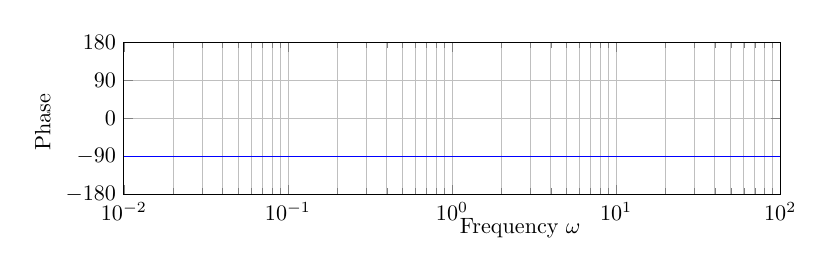
\begin{tikzpicture}
        [
            scale = 0.8,
            >=latex
        ]
        \begin{axis}
            [
                width=12cm,
                height=4cm,
                xmode=log,
                xmin=0.01, xmax=100, ymin=-180, ymax=180,
                x label style={anchor=west},
                xlabel=Frequency $\omega$,
                y label style={anchor=south},
                ylabel=Phase $\degree$,
                ytick={-180, -90, 0, 90, 180},
                % yticklabels={-180, -90, 0, 90, 180},
                xmajorgrids=true,
                xminorgrids=true,
                ymajorgrids=true
            ]
            
            % Phase
            \addplot[thick, color=blue, domain=0.01:100]{-90};
                
        \end{axis}
            
    \end{tikzpicture}
\end{center} 


\subsection{Bodediagramm eines Differenzierer}

Ein Differenzierer mit $G(s) = K \cdot s$ hat eine Nullstelle bei der Frequenz $\omega = 0$. Im Bodediagramm wird der Differenzierer so
dargestellt, dass bei Frequenz $\omega = 1$ die Verstärkung $20 \, \deci \bel \cdot \log_{10}(K)$ erreicht ist.
Die Steigung beträgt $20 \, \deci \bel / \mathrm{Dek}$ und die Phase ist konstant bei $\varphi = \frac{\pi}{2}$

\begin{center}
    % Gain
    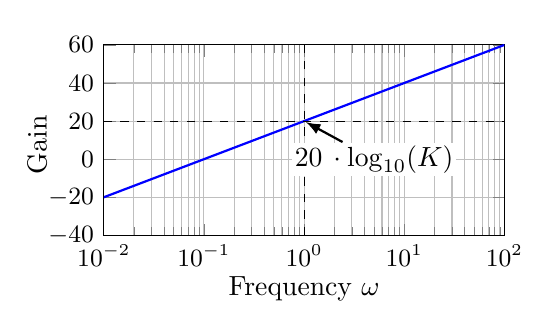
\begin{tikzpicture}
        [%
            scale = 1,
            >=latex
        ]
        \begin{axis}
            [%
                width=.55\columnwidth,
                height=4cm,
                % tick label style
                tick label style={font=\small},
                % x-axis
                xmode=log,
                xmin=0.01, xmax=100, ymin=-40, ymax=60,
                x label style={anchor=north, inner sep=0pt},
                xlabel=Frequency $\omega$,
                xmajorgrids=true,
                xminorgrids=true,
                % y-axis
                y label style={yshift=-1mm, anchor=south, inner sep=0pt},
                ylabel=Gain $\deci \bel$,
                ymajorgrids=true,
                yminorgrids=false
            ]
            % Plot
            \addplot[thick, color=blue, domain=0.01:100]{+20*log10(x)+20};
            
            % guide lines
            \addplot[dashed, color=black, domain=0.01:100]{20}; 
            \addplot [dashed, color=black] coordinates {(1, -40) (1, 60)};
           
            % Node / Label
            \node[inner sep=0pt] (p) at (1, 20) {};
            \node[fill=white, inner sep=1pt] (q) at (5, 0) {$20 \, \deci \bel \cdot \log_{10}(K)$};

            \draw[->, thick, color=black] (q) -- (p);
        \end{axis}
    \end{tikzpicture}
    % Phase
    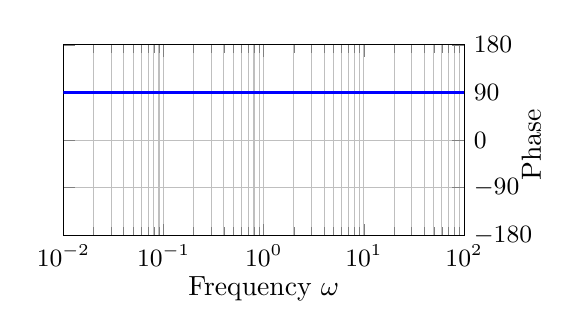
\begin{tikzpicture}
        [%
            scale = 1,
            >=latex
        ]
        \begin{axis}
            [%
                width=.55\columnwidth,
                height=4cm,
                % tick label style
                tick label style={font=\small},
                % x-axis
                xmode=log,
                xmin=0.01, xmax=100, ymin=-180, ymax=180,
                x label style={anchor=north, inner sep=0pt},
                xlabel=Frequency $\omega$,
                xmajorgrids=true,
                xminorgrids=true,
                % y-axis
                y label style={anchor=south, inner sep=0pt},
                ylabel=Phase $\degree$,
                yticklabel pos=right,
                ytick={-180, -90, 0, 90, 180},
                ymajorgrids=true,
                yminorgrids=false
            ]
            
            % Phase
            \addplot[thick, color=blue, domain=0.01:100]{90};
        \end{axis}
    \end{tikzpicture}
\end{center}

 


\subsection{z-Transformation}
\label{z-Transformation}

Die z-Transformation wird verwendet, um \textbf{diskrete} Signale in den Frequenzbereich zu transformieren.

\renewcommand{\arraystretch}{1}

\begin{center}
    \begin{tabular}{c c}
        \toprule
        \textbf{Zeitbereich}    & \textbf{Frequenzbereich}  \\
        \toprule
        \strut$u(k)$                  & $U(z)$                    \\
        \strut$u(k-1)$                & $z^{-1} \cdot U(z) = \frac{1}{z} \cdot U(z)$ \\
        \strut$u(k+1)$                & $z \cdot U(z)$\\
        \bottomrule
    \end{tabular}
\end{center}


\subsubsection{Z-Transformation mit Matlab}

\lstinputlisting{snippets/z_transformation.m}


\subsection{Fourier- bzw. Laplace-Transformation}

Die Fourier- und die Laplace-Transformation werden verwendet, um \textbf{kontinuierliche} Signale ein den Frequenzbereich zu transformieren.

\begin{center}
    \begin{tabular}{c c c}
        \toprule
        \textbf{Zeitbereich}                  & \textbf{Frequenzbereich (Fourier)}                & \textbf{Frequenzbereich (Laplace)}      \\
        \toprule
        \strut$u(t)$                          & $U(\jimg \omega)$                                 & $U(s)$                                  \\
        \strut$\int u(\tau) \, \diff \tau$    & $\frac{1}{\jimg \omega} \cdot U(\jimg \omega)$    & $\frac{1}{s} \cdot U(s)$                \\
        \strut$\frac{\diff}{\diff u(t)}$      & $\jimg \omega \cdot U(\jimg \omega)$              & $s \cdot U(s)$                          \\
        \strut$u(t \pm T_0)$                  & $U(\jimg \omega) \cdot e^{\pm \jimg \omega T_0}$  & $U(s) \cdot e^{\pm s T_0}$                          \\
        \bottomrule
    \end{tabular}
\end{center}
\renewcommand{\arraystretch}{1}



\section{Statische Grundglieder (ohne Gedächtnis)}

Der Ausgang des Systems ist \textbf{nur} vom aktuellen Eingang abhängig 
$$ y(t) = f( u(t) ) $$
\textbf{Hinweis:} $u(t)$ entspricht meist $A \cdot \varepsilon(t)$ (skalierter Einheitssprung)


\subsection{P-Glied (Proportional)}{26}

$$ \boxed{ y(t) = K \cdot u(t) } $$

\begin{minipage}{0.23\columnwidth}
    \includegraphics[width=0.8\columnwidth]{images/eingangssignal_schrittantwort} 
\end{minipage}
\hfill
\begin{minipage}{0.23\columnwidth}
    \includegraphics[width=0.8\columnwidth]{images/schrittantwort_p-glied} 
\end{minipage}
\hfill
\begin{minipage}{0.23\columnwidth}
    \includegraphics[width=0.8\columnwidth]{images/symbol_p-glied_1}
\end{minipage}
\hfill
\begin{minipage}{0.23\columnwidth}
    \includegraphics[width=0.8\columnwidth]{images/symbol_p-glied_2}
\end{minipage}


\section{Dynamische Grundglieder (mit Gedächtnis)}

Der Ausgang des Systems ist vom aktuellen \textbf{und} von vergangenen Eingängen abhängig.
Vergangene Eingänge werden im System in einem Speicher, einem Zustand $x(t)$ abgelegt. 
$$ y(t) = f( u(t), \, x(t) ) $$


\subsubsection{Prozesse mit / ohne Ausgleich}

\begin{tabular}{ll}
ohne Ausgleich:     & Sprungantwort wächst grenzenlos an \\
mit Ausgleich:      & Sprungantwort strebt gegen endlichen Wert \\
				    & \textrightarrow\ \textbf{Gegenkopplung} am Ausgang
\end{tabular}


\subsection{Totzeit-Glied}{30}

$$ \boxed{ y(t) =  u(t - T_t) }  $$

\includegraphics[width=0.9\columnwidth]{images/totzeit-glied}


\subsection{I-Glied (Integrierer)}{29}

\begin{minipage}{0.48\columnwidth}
    $$ \boxed{ \text{DGL: } \dot{y}(t) = K \cdot u(t) }  $$
\end{minipage}
\hfill
\begin{minipage}{0.48\columnwidth}
    $$ \boxed{ \scriptstyle{ y = \int\limits_{- \infty}^t u(\tau) \, d \tau = K \int\limits_{- \infty}^t u(\tau) \, d \tau + y(0) } }$$
\end{minipage}

\includegraphics[width=0.9\columnwidth]{images/i-glied} 


\subsection[PT1-Glied]{$\text{PT}_1$-Glied}{31-33}

Ein Energiespeicher \textrightarrow\ System schwingt nicht

\begin{minipage}{0.48\columnwidth}
    $$ \boxed{ \text{DGL: } T \, \dot{y}(t) + y(t) = K \cdot u(t) }  $$
\end{minipage}
\hfill
\begin{minipage}{0.48\columnwidth}
    $$ \boxed{ y(t) = K \, A + (y_0 - K \, A) \cdot e^{- \frac{t}{T}} } $$
\end{minipage}


\begin{minipage}{0.5\columnwidth}
    \includegraphics[width=\columnwidth]{images/pt1-glied_kennlinie}
\end{minipage}
\hfill
\begin{minipage}{0.4\columnwidth}
    \includegraphics[width=0.8\columnwidth]{images/symbol_PT1-glied}
\end{minipage}


\subsubsection{Modellierung einer $\text{PT}_1$ Regelstrecke}

\begin{itemize}
    \item Ausmessen der Sprungantwort $u(t) = A \cdot \varepsilon(t)$ \\
        \textrightarrow\ Die Sprungantwort entspricht dem Diagramm
    \item Parameter $K$ berechnen: $K = \frac{y_\infty}{A}$ 
    \item Parameter $T$ bestimmen: Tangente am Anfang durch Punkt $P$ \\
        oder: Zeit bis $y(T) = 0.63 \cdot K \, A$ erreicht ist \textrightarrow\ $T$ ablesen
\end{itemize}


\example{Beispiel $\text{PT}_1$-Glied als Blockschaltbild}

\begin{minipage}{0.48\columnwidth}
    \includegraphics[width=\columnwidth]{images/pT1_blockschaltbild}
\end{minipage}
\hfill
\begin{minipage}{0.48\columnwidth}
    $$ \boxed{ \text{Allg: } T \, \dot{y}(t) + y(t) = K \cdot u(t) }  $$
    $$ \boxed{ \text{Bsp: } RC \, \dot{u}(t) + u(t) = R \cdot i(t) }  $$
\end{minipage}


\example{{Beispiel $\text{PT}_1$-Glied vs. $\text{DT}_1$-Glied}}

\begin{minipage}{0.48\columnwidth}
    \begin{center}
        \myul{$\boldsymbol{\text{PT}_1}$-Glied}
    \end{center}
    \includegraphics[width=0.98\columnwidth]{images/pT1_blockschaltbild_2}
\end{minipage}
\hfill
\begin{minipage}{0.48\columnwidth}
    \begin{center}
        \myul{$\boldsymbol{\text{DT}_1}$-Glied}
    \end{center}
    \includegraphics[width=0.98\columnwidth]{images/DT1-glied_blockschaltbild}
\end{minipage}


\subsection[PT2-Glied]{$\text{PT}_2$-Glied}{34}

Zwei Energiespeicher \textrightarrow\ \textbf{System kann schwingen}

\begin{minipage}{0.4\columnwidth}
    $$ \boxed{ \text{DGL: } T^2 \cdot  \ddot{y} + 2 \, \zeta \, T \cdot \dot{y} + y = K \cdot u } $$
\end{minipage}
\hfill
\begin{minipage}{0.58\columnwidth}
    $$ \boxed{ y(t) = K \: A \big[ 1 + e^{\sigma t} \big( - \cos(\omega t) + \frac{\sigma}{\omega} \sin(\omega t)  \big)  \big] }  $$
\end{minipage}


\begin{minipage}{0.55\columnwidth}
    \includegraphics[width=\columnwidth]{images/pT2_sprungantwort}
\end{minipage}
\hfill
\begin{minipage}{0.38\columnwidth}
    \includegraphics[width=0.75\columnwidth]{images/pT2_symbol} 

    \begin{center}
        $ \omega = \omega_n \cdot \sqrt{1 - \zeta^2} $ \\
        $y_m = e^h \cdot y_{\infty}$ \\
    \end{center}
\end{minipage}


\begin{tabular}{c c c}
    $ K = \frac{y_{\infty}}{A}$                                                     & $ h = \ln \big( \frac{y_m}{y_{\infty}} \big)$                                 & $ \omega = \frac{2 \, \pi}{T_{\omega}} = \frac{\pi}{T_m} $ \\

    \rule{0pt}{10pt}$ \sigma = \frac{h \, \omega}{\pi} = - \omega_n \cdot \zeta$    & $ \omega_n = \sqrt{\omega^2 + \sigma^2} = - \frac{\sigma}{\zeta}$             & $ \zeta = - \frac{h}{\sqrt{h^2 + \pi^2}} $ \\

    \rule{0pt}{10pt}$T = \frac{1}{\omega_n}$                                        & $T_{KA} = T_M - \frac{1}{\omega} \arctan \big(  \frac{\omega}{\sigma} \big)$  & $y(T_{KA}) = K \: A$ \\
\end{tabular}


\subsection{D-Glied (Idealer Differenzierer)}{37}

$$ \boxed{  y(t) = K \cdot \frac{\diff u(t)}{\diff t} = K  \cdot \dot{u}(t) } $$

\begin{minipage}{0.25\columnwidth} 
    \center 
    \myul{ideal}  \\
    \includegraphics[width=0.65\columnwidth]{images/D-glied_ideal}
\end{minipage}
\hfill
\begin{minipage}{0.25\columnwidth}
    \center 
    \myul{real} \\
    \includegraphics[width=0.6\columnwidth]{images/D-glied_real}
\end{minipage}
\hfill
\begin{minipage}{0.25\columnwidth}
    \includegraphics[width=0.9\columnwidth]{images/D-glied_symbol}
\end{minipage}


\subsection[DT1-Glied (Realisierbarer Differenzierer)]{$\text{DT}_1$-Glied (Realisierbarer Differenzierer)}{38}

\begin{minipage}{0.48\columnwidth}  
    $$ \boxed{ w(t) = A \cdot (1 - e^{-\frac{t}{T}}) } $$
\end{minipage}
\hfill
\begin{minipage}{0.48\columnwidth}
    $$ \boxed{ y(t) = \frac{K \cdot A}{T} \,  e^{-\frac{t}{T}} } $$
\end{minipage}

\includegraphics[width=\columnwidth]{images/DT1-glied}


\subsection{Lead-Glied / Lag-Glied / Lead-Lag-Glied}{40-41}

Lead-/ Lag-Glieder sind zwei Varianten von $\text{PDT}_1$-Gliedern. 

\begin{tabular}{ll}
    Lead:   & $K_P$ und $K_D$ haben \textbf{gleiches} Vorzeichen \\
    Lag:    & $K_P$ und $K_D$ haben \textbf{unterschiedliches} Vorzeichen \\
\end{tabular}

Lead- und Lag-Glieder können auch als Parallelschaltungen eines P- und eines $\text{PT}_1$-Glieds aufgefasst werden. 
Das Lead-Lag-Glied ist eine Serieschaltung aus Lead- und Lag-Glied.

\begin{minipage}{0.45\columnwidth}
    \center
    \myul{Lead-Glied}
    \includegraphics[width=0.9\columnwidth]{images/lead-glied}
\end{minipage}
\hfill
\begin{minipage}{0.45\columnwidth}
    \center
    \myul{Lag-Glied} 
    \includegraphics[width=0.9\columnwidth]{images/lag-glied}
\end{minipage}

